% Copyright 2004 by Till Tantau <tantau@users.sourceforge.net>.
%
% In principle, this file can be redistributed and/or modified under
% the terms of the GNU Public License, version 2.
%
% However, this file is supposed to be a template to be modified
% for your own needs. For this reason, if you use this file as a
% template and not specifically distribute it as part of a another
% package/program, I grant the extra permission to freely copy and
% modify this file as you see fit and even to delete this copyright
% notice. 

\documentclass[xcolor=table]{beamer}

\usepackage{pgfbaseimage}
\usepackage{multicol}

% There are many different themes available for Beamer. A comprehensive
% list with examples is given here:
% http://deic.uab.es/~iblanes/beamer_gallery/index_by_theme.html
% You can uncomment the themes below if you would like to use a different
% one:
%\usetheme{AnnArbor}
%\usetheme{Antibes}
%\usetheme{Bergen}
%\usetheme{Berkeley}
%\usetheme{Berlin}
%\usetheme{Boadilla}
%\usetheme{boxes}
%\usetheme{CambridgeUS}
%\usetheme{Copenhagen}
%\usetheme{Darmstadt}
%\usetheme{default}
%\usetheme{Frankfurt}
%\usetheme{Goettingen}
%\usetheme{Hannover}
%\usetheme{Ilmenau}
%\usetheme{JuanLesPins}
%\usetheme{Luebeck}
\usetheme{Madrid}
%\usetheme{Malmoe}
%\usetheme{Marburg}
%\usetheme{Montpellier}
%\usetheme{PaloAlto}
%\usetheme{Pittsburgh}
%\usetheme{Rochester}
%\usetheme{Singapore}
%\usetheme{Szeged}
%\usetheme{Warsaw}

\title[Feature addition to Bodhitree]{Enhancement of Bodhitree through the}

% A subtitle is optional and this may be deleted
\subtitle{Development of Additional Features}

\author{Avijeet Gaikwad \\ 143050101}

\institute[] % (optional, but mostly needed)
{  Guided by \\
	\vspace{0.1cm}
	{\small Prof. Kameswari Chebrolu} \\
	\vspace{0.5cm}
	Department of Computer Science and Engineering\\
	IIT Bombay
}

\date{27th June, 2016}
% - Either use conference name or its abbreviation.
% - Not really informative to the audience, more for people (including
%   yourself) who are reading the slides online

\subject{Theoretical Computer Science}
% This is only inserted into the PDF information catalog. Can be left
% out. 

% If you have a file called "university-logo-filename.xxx", where xxx
% is a graphic format that can be processed by latex or pdflatex,
% resp., then you can add a logo as follows:

\pgfdeclareimage[height=0.5cm]{university-logo}{./media/iitb.jpg}
\logo{\pgfuseimage{university-logo}}

% Delete this, if you do not want the table of contents to pop up at
% the beginning of each subsection:

%\AtBeginSection[]
%{
%  \begin{frame}<beamer>{Outline}
%  	\begin{multicols}{2}
%	  \tableofcontents[currentsection]
%	\end{multicols}
%  \end{frame}
%}
%
%\AtBeginSubsection[]
%{
%  \begin{frame}<beamer>{Outline}
%  	\begin{multicols}{2}
%	  \tableofcontents[currentsection,currentsubsection]
%	\end{multicols}
%  \end{frame}
%}

% Let's get started
\begin{document}

\begin{frame}
  \titlepage
\end{frame}

\begin{frame}{Outline}
  \begin{multicols}{2}
    \tableofcontents
  \end{multicols}
  % You might wish to add the option [pausesections]
\end{frame}

% Section and subsections will appear in the presentation overview
% and table of contents.
\section{Bodhitree}

\subsection{Introduction}

\begin{frame}{Bodhitree}{Introduction and Details}
  \begin{itemize}
  \item {
    Bodhitree is an e-learning platform
    \begin{itemize}
    	\item Design to mimic classroom setting
    	\item Host multimedia textbooks
    \end{itemize}
  }
  \item {
    Types of users:
    \begin{itemize}
    	\item Instructor
    	\item Student
    \end{itemize}
  }
  \item {
  	Types of courses
	\begin{itemize}
		\item Bodhi-class
		\item Bodhi-book
	\end{itemize}
  }
\end{itemize}
\end{frame}

\subsection{Courses: Bodhi-class and Bodhi-book}

% You can reveal the parts of a slide one at a time
% with the \pause command:
\begin{frame}{Bodhi-class}{A flipped classroom model}
	\begin{figure}
	\centering
	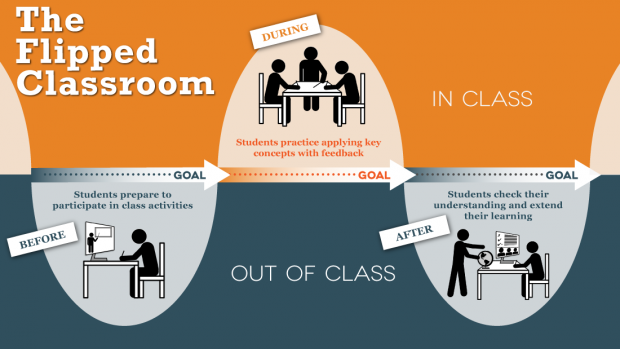
\includegraphics[width=0.8\linewidth]{./media/flippedflowmodel}\\[-1ex]
	\hspace*{-1in}{\tiny Source:\cite{flipped} The University of Texas at Austin: Faculty Innovation Center}
	\caption{Flipped classroom model}
	\label{fig:btclass}
	\end{figure}
\end{frame}

\begin{frame}{Bodhi-book}{A multimedia textbook model}
	\begin{figure}
	\centering
	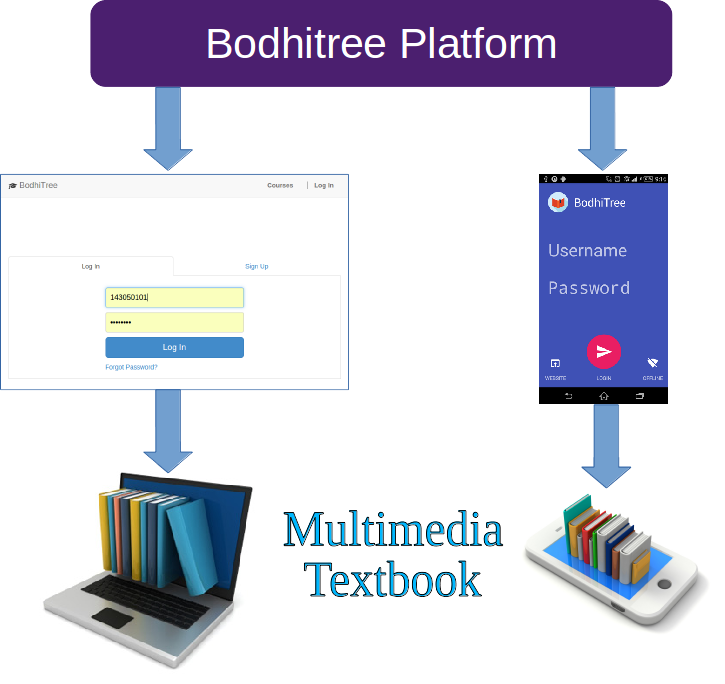
\includegraphics[width=0.5\linewidth]{./media/bmmt}\\[-1ex]
	\caption{Multimedia textbook model}
	\label{fig:btmmb}
	\end{figure}
\end{frame}

\subsection{Components}

\begin{frame}{Overview of the components that constitute Bodhitree}
  	\begin{itemize}
  		\item Courseware
  		\begin{itemize}
  			\item Chapters
  			\item Concepts
  			\item Progress
  		\end{itemize}
		\item Learning elements
		\begin{itemize}
  			\item Videos
	 		\item Quiz
	 		\begin{itemize}
	 			\item In-video quiz
	 			\item Out of video quiz
	 		\end{itemize}
	 		\item Documents			
		\end{itemize}	
  		\item Interaction
  		\begin{itemize}
  			\item Discussion forums
  			\item Chat
  		\end{itemize}
  		\item Labs
  		\begin{itemize}
	  		\item Report grading
	  		\item Assignments
  		\end{itemize}
  	\end{itemize}
\end{frame}

\subsection{Development details}

\begin{frame}{Development details}
	\begin{itemize}
		\item Django web framework (Back-end)
		\begin{itemize}
			\item (M) Designing the model
			\item (V) Creating the templates
			\item (C) Writing the views and mapping the URLs
		\end{itemize}
		\vspace{0.2in}
		\item React.js (Front-end)
		\begin{itemize}
			\item Component based design
			\item Virtual DOM
		\end{itemize}
	\end{itemize}
\end{frame}

\section{Objective and Overview}

\subsection{Motivation}

\begin{frame}{Objective and Motivation}
	\begin{itemize}
		\item Objective is to enhance the Bodhitree platform through the addition of new features
		\item Need for new features, development ideas:
		\begin{itemize}
			\item Instructor requirements
			\item Student's and Instructor's feedback
			\item Brainstorming sessions
		\end{itemize}
		\item Classification of features pertaining to:
		\begin{itemize}
			\item Bodhi-class
			\item Bodhi-flipped
			\item General
		\end{itemize}
	\end{itemize}
\end{frame}

\subsection{Overview of the work}

\begin{frame}{Classification and Overview of the work}
	\begin{itemize}
		\item Bodhi-class
		\begin{itemize}
			\item Marks for offline exams
			\item Archiving emails
		\end{itemize}
		\item Bodhi-book
		\begin{itemize}
			\item Prerequisites and course graph
			\item Access control
		\end{itemize}
		\item General
		\begin{itemize}
			\item Facebook style notifications
			\item Miscellaneous
			\begin{itemize}
				\item In-video quizzes ON/OFF
				\item Setting importance to threads
				\item Email instructors when a new thread is added
			\end{itemize}
		\end{itemize}
	\end{itemize}
\end{frame}

\section{Bodhi-class}

\subsection{Marks for offline examinations}

\begin{frame}{Marks for offline examinations}
	\begin{block}{Problem Statement}
		\begin{itemize}
			\item Several offline exams are conducted in the Bodhi-class model
			\item The marks for these offline exams are usually sent by emails, having CSV files attachments
			\item It is required to have an interface to display these marks to the students on Bodhitree itself
		\end{itemize}
	\end{block}
\end{frame}

\begin{frame}{Specifications}
	\textbf{Instructor Specifications}
	\begin{itemize}
		\item Upload a CSV containing the students marks
		\item The file should have the exam details and marks, along with the usernames of the students, in the following format
	\end{itemize}

	\textbf{Students Specifications}
	\begin{itemize}
		\item Students must be able to view only their marks that are uploaded for the course
	\end{itemize}
	
\end{frame}

\begin{frame}{Design}{User Interface: Instructor}
	\textbf{User Interface as seen by the instructor}
	\begin{figure}
		\centering
		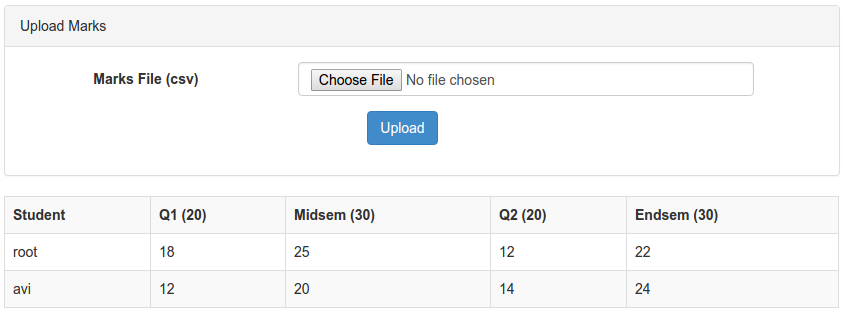
\includegraphics[width=0.8\linewidth]{media/marksi}
		\caption{Instructor's view of CSV upload and display of students marks}
		\label{fig:marksi}
	\end{figure}
\end{frame}

\begin{frame}{Design}{User Interface: Student}
	\textbf{User Interface as seen by the student}
	\begin{figure}
		\centering
		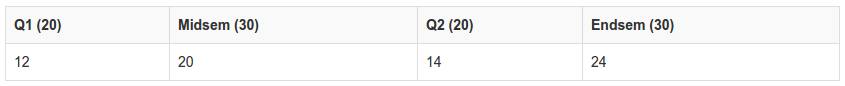
\includegraphics[width=0.8\linewidth]{media/markss1}
		\caption{Student 2's view of his marks}
		\label{fig:markss1}
	\end{figure}
\end{frame}

\begin{frame}{Design}{Upload of marks}
	\textbf{Uploading CSV file}
	
	\begin{center}
		\rowcolors{1}{}{lightgray}
		\bgroup
		\def\arraystretch{1.5}
		\begin{tabular}{ccccc}
			\hline
			\textbf{EXAM\_TYPE} & Q1 & Midsem & Q2 & Endsem \\
			\textbf{MAX\_MARKS} & 20 & 30 & 20 & 30 \\
			Student 1 & 18 & 25 & 12 & 22 \\ 
			Student 2 & 12 & 20 & 14 & 24 \\ 
			\hline 
		\end{tabular}
		\egroup
	\end{center}
		
\end{frame}


\begin{frame}{Design}{Storage of marks}
	\textbf{Storing marks in the database}
	\begin{figure}
		\centering
		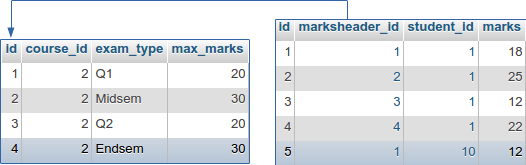
\includegraphics[width=0.8\linewidth]{media/marksdb} \\
		\hspace{1.2cm}Exams details \hspace{1.5cm} Marks obtained by students
		\caption{Data view of the marks module}
		\label{fig:marksdb}
	\end{figure}
	
\end{frame}

\subsection{Archiving of emails}

\begin{frame}{Archiving of emails}
	\begin{block}{Problem Statement}
		\begin{itemize}
			\item Instructors frequently send emails in the Bodhi-class
			\item These emails are concerned with important announcements and updates in the course
			\item No easy way for the instructor to view the emails
			\item Need for archiving and course-wise categorization
		\end{itemize}
	\end{block}
\end{frame}

\begin{frame}{Specifications}
	\begin{itemize}
		\item All the emails sent by the instructors must be archived
		\item Instructor should be able to view all the emails sent by him in a particular course
		\item Student must be able to view all the emails that are received by him
		\item Sorting and searching features should be available
	\end{itemize}
\end{frame}

\begin{frame}{Design}{Archiving the emails}
	\textbf{Archiving the emails}
	\begin{itemize}
		\item Function \textit{archive\_mail()} called whenever an email is sent
		\item Foreign keys to the current \textit{user}, \textit{course} and \textit{list of recipients} (many to many relation)
		\item Postgres automatically adds the current date and time
	\end{itemize}
\end{frame}

\begin{frame}{Design}{Displaying the archived emails}
	\textbf{Displaying the archived emails}
	\begin{itemize}
		\item User makes an AJAX request to the server
		\item Server checks the dtails of the user in the current session 
		\item Data is fetched in JSON format
	\end{itemize}
	\begin{figure}
		\centering
		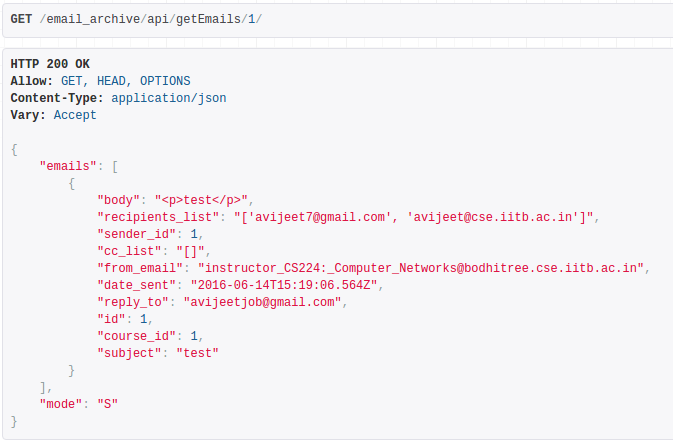
\includegraphics[width=0.6\linewidth]{media/email_json} \\
		\label{fig:email_json}
	\end{figure}
\end{frame}

\begin{frame}{Design}{UI for viewing the emails}
	\textbf{UI for viewing the emails}
	\begin{itemize}
		\item Component based design using React.js
		\item Sorted by most recent first
	\end{itemize}
	\begin{figure}
		\centering
		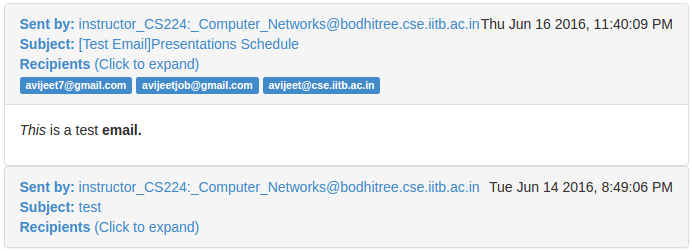
\includegraphics[width=0.8\linewidth]{media/email_ui} \\
		\label{fig:email_ui}
	\end{figure}
\end{frame}

\begin{frame}{Design}{Search and filter functions}
	\textbf{Search and filter functions}
	\begin{itemize}
		\item Searchbox and date filter
		\item \textit{Instant search}
	\end{itemize}
	\begin{figure}
		\centering
		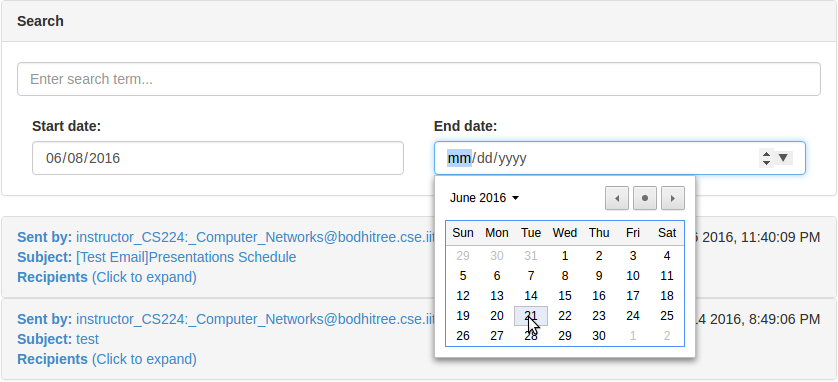
\includegraphics[width=0.8\linewidth]{media/email_search} \\
		\label{fig:email_search}
	\end{figure}
\end{frame}

\section{Bodhi-book}

\subsection{Prerequisites and course graph}

\begin{frame}{Prerequisites and course graph}
	\begin{block}{Problem Statement}
		\begin{itemize}
			\item Bodhi-book model lacks significant involvement of instructors
			\item Dependencies in chapters and concepts
			\item Proficiency levels required for complete understanding
			\item Guidelines are necessary for students
			\item Graphical representation of the course and the guidelines help the students to progress in a better way
		\end{itemize}
	\end{block}
\end{frame}

\begin{frame}{Specifications}
	\textbf{Motivation is to ensure that every student has the required background knowledge before attempting to learn a new concept}
	\begin{itemize}
		\item Instructor specifies prerequisites for a concept
		\item Prerequisites viewable on the concept page
		\item Graph generated using the course data, which serves as a guideline
		\item Instructor modifies and finalizes the course graph
	\end{itemize}	
\end{frame}

\begin{frame}{Design}{Storing the prerequisites}
	\textbf{Storing the prerequisites}
	\begin{itemize}
		\item Concepts/Chapters are the prerequisites for other Concepts/Chapters
		\item Prerequisites are stored as a list of Concept/Chapter id's
		\item Default values are a blank list \textit{[ ]}
		\item In case of a Chapter, a \textit{``g''} character is appended in front of the id
		\item Example of prerequisites data for a concept: \\
		\textit{[``g1'',``5'',``6'']}
	\end{itemize}
\end{frame}

\begin{frame}{Design}{UI to add prerequisites}
	\begin{itemize}
		\item Only the instructor has authority
		\item Concepts categorized into chapters
		\item Component based design, immediate request
	\end{itemize}
	\begin{figure}
		\centering
		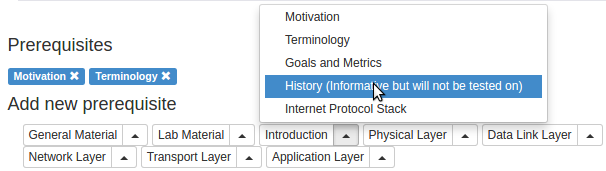
\includegraphics[width=0.6\linewidth]{media/add_prereq}
		\caption{Adding prerequisite to a concept}
		\label{fig:add_prereq}
%		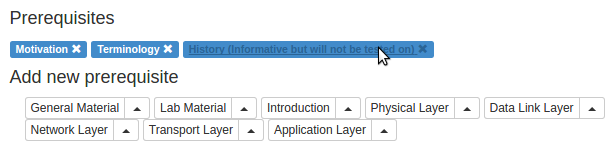
\includegraphics[width=0.6\linewidth]{media/remove_prereq}
%		\caption{Removing prerequisite from a concept}
%		\label{fig:remove_prereq}		
	\end{figure}
\end{frame}

\begin{frame}{Design}{Student's view of prerequisites}
	\textbf{Student's view of prerequisites on the concept page}
	\begin{figure}
		\centering
		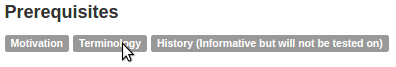
\includegraphics[width=0.5\linewidth]{./media/prereq_stud}
		\label{fig:prereq_stud}
	\end{figure}
	\begin{itemize}
		\item Navigable links
	\end{itemize}
\end{frame}

\begin{frame}{Design}{Creation of the course graph}
Several graph generation libraries used to generate initial course graphs:
	\begin{itemize}
		\item \textbf{Graphviz:} Python library which generates an image of the final graph, non-interactive
		\item \textbf{Arbor.js:} Javascript library which dynamically generates interactive graphs, allows users to interact with the components
		\item \textbf{Vis.js:} Javascript library, interactive graphs, GUI to create/modify existing graphs
	\end{itemize}
\end{frame}

\begin{frame}{Design}{Graphviz}
\textbf{Graph generated using Graphviz library}
	\begin{figure}
		\centering
		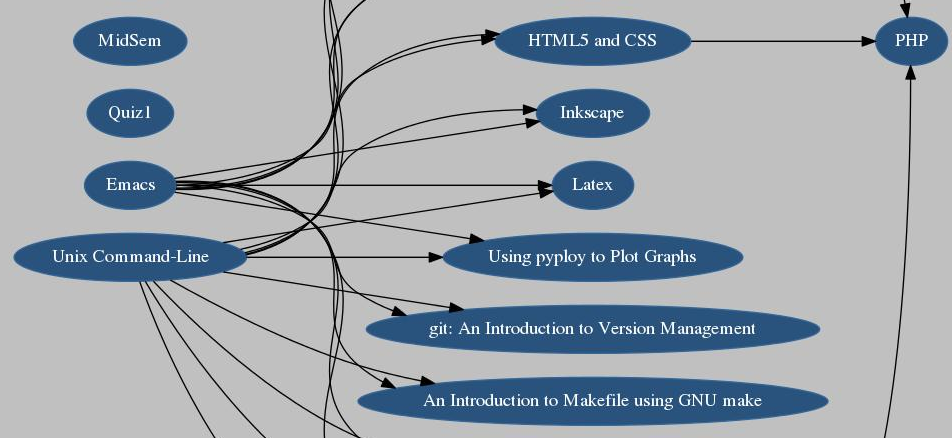
\includegraphics[width=0.8\linewidth]{media/Graphviz}
		\caption{Part of a complex graph generated using graphviz}
		\label{fig:Graphviz}
	\end{figure}
\end{frame}

\begin{frame}{Design}{Arbor.js}
\textbf{Graph generated using Arbor.js}
	\begin{figure}
		\centering
		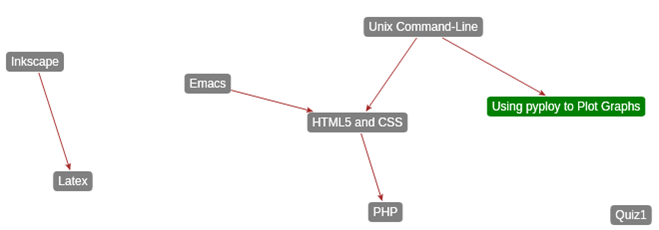
\includegraphics[width=0.8\linewidth]{media/PrereqGraph}
		\caption{Part of a graph generated using arbor.js}
		\label{fig:PrereqGraph}
	\end{figure}
\end{frame}

\begin{frame}{Design}{Vis.js}
\textbf{Graph generated using Vis.js}
	\begin{figure}
		\centering
		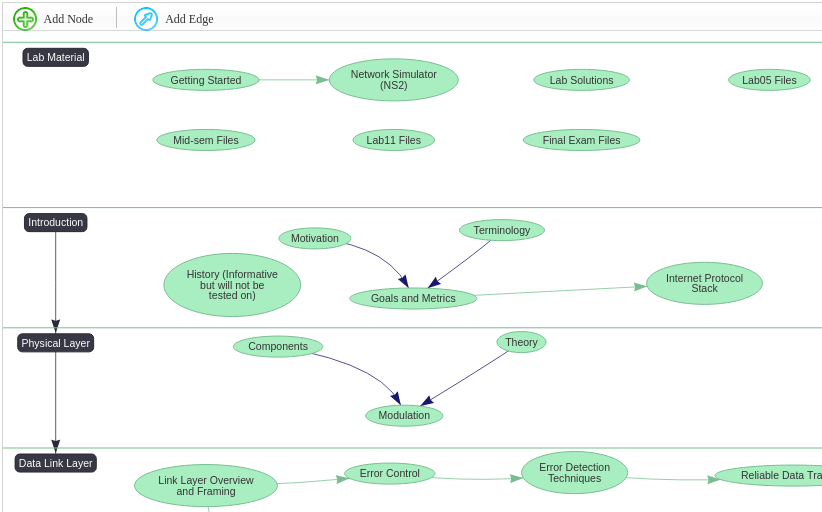
\includegraphics[width=0.8\linewidth]{media/vis_js}
%		\caption{Using Vis.js}
		\label{fig:vis_js}
	\end{figure}
\end{frame}

\begin{frame}{Design}{Creation of graph using vis.js}
	\begin{itemize}
		\item Function created to fetch the course data, convert it to JSON and render the graph (html file)
		\item JSON captured on the client side. Function for creation and organization of nodes and edges written in JavaScript
		\item Instructor must save the graph before the student can view it
		\item All the components on the canvas are interactive and modifiable
		\item Example of Nodes and Edges data: \\
		\begin{table}[H]
			\centering
			\begin{tabular}{l|l}
				\hline \textbf{Nodes} & \textbf{Edges} \\ 
				\hline\hspace{-0.1cm}[\{id: 1, label: 'Node 1'\}, & \hspace{-0.1cm}[\{from: 1, to: 3\}, \\
				\{id: 2, label: 'Node 2'\}, & \{from: 1, to: 2\}, \\
				\{id: 3, label: 'Node 3'\}, & \{from: 2, to: 4\}, \\
				\{id: 4, label: 'Node 4'\}, & \{from: 2, to: 5\}] \\
				\{id: 5, label: 'Node 5'\}] & \\
				\hline 
			\end{tabular} 
		\end{table}
	\end{itemize}
\end{frame}

\begin{frame}{Future work}{Ideas to empower course graphs}
	\begin{itemize}
		\item Using data from the progress module to display proficiency levels of students
		\item Generating dynamic, student specific graphs for providing alternative learning paths
		\item Creating multidimensional graphs, which display in-depth information and provide navigation to courseware elements
	\end{itemize}
\end{frame}

\subsection{Access control}

\begin{frame}{Access control}{Motivation}
	\textbf{Providing differential access to users towards the content}
	\begin{figure}
	\centering
	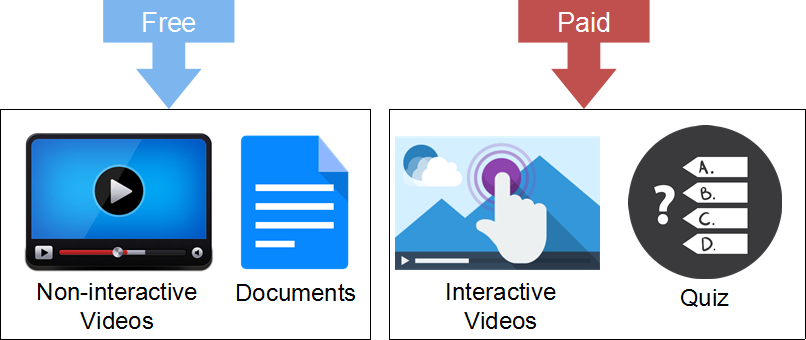
\includegraphics[width=0.6\linewidth]{media/AccessControl}
	\label{fig:AccessControl}
	\end{figure}
	\begin{block}{Problem Statement}
		\begin{itemize}
			\item Giving the instructor authority to limit the access a student has to the content in his course
		\end{itemize}
	\end{block}
\end{frame}

\begin{frame}{Specifications}{Concept of locks and keys}
	\textbf{8 doors, 4 users, 1 owner, 4 types of locks and their keys}
	\begin{figure}
		\centering
		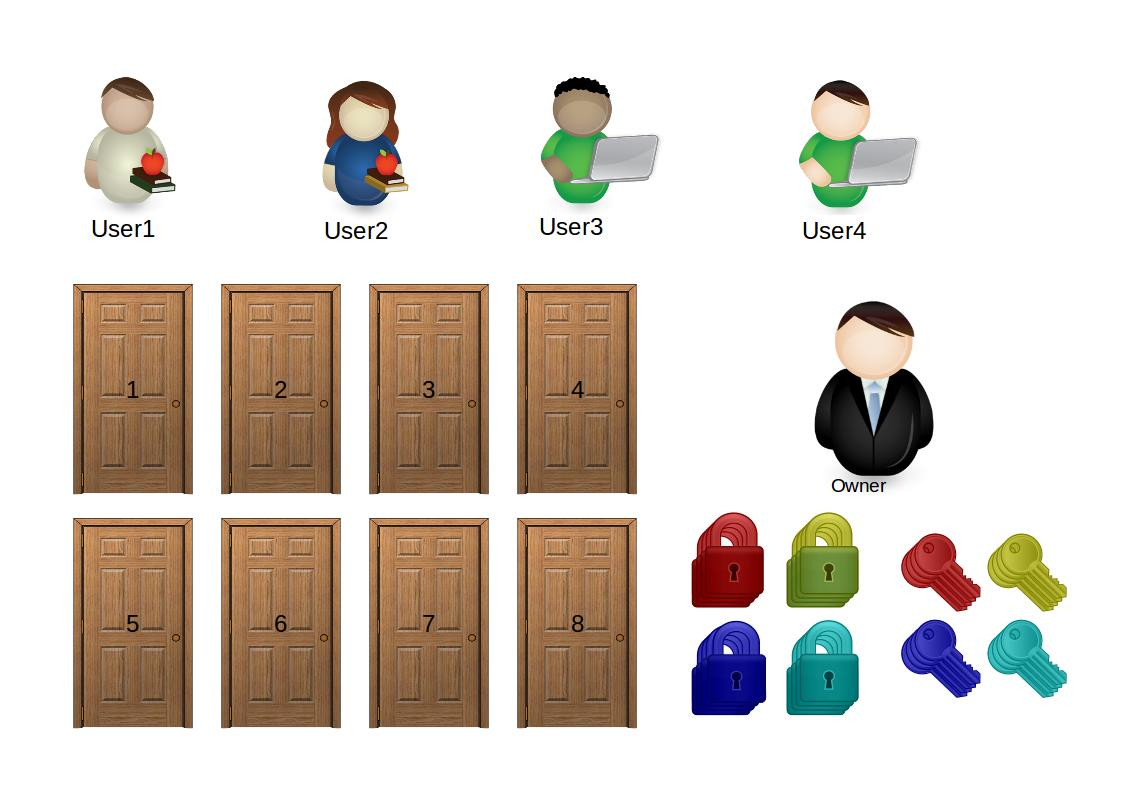
\includegraphics[width=0.7\linewidth]{./media/1}
		\label{fig:1}
	\end{figure}
\end{frame}

\begin{frame}{Specifications}{Concept of locks and keys}
	\textbf{Owner locks door no. 8, thus restricting access to it}
	\begin{figure}
		\centering
		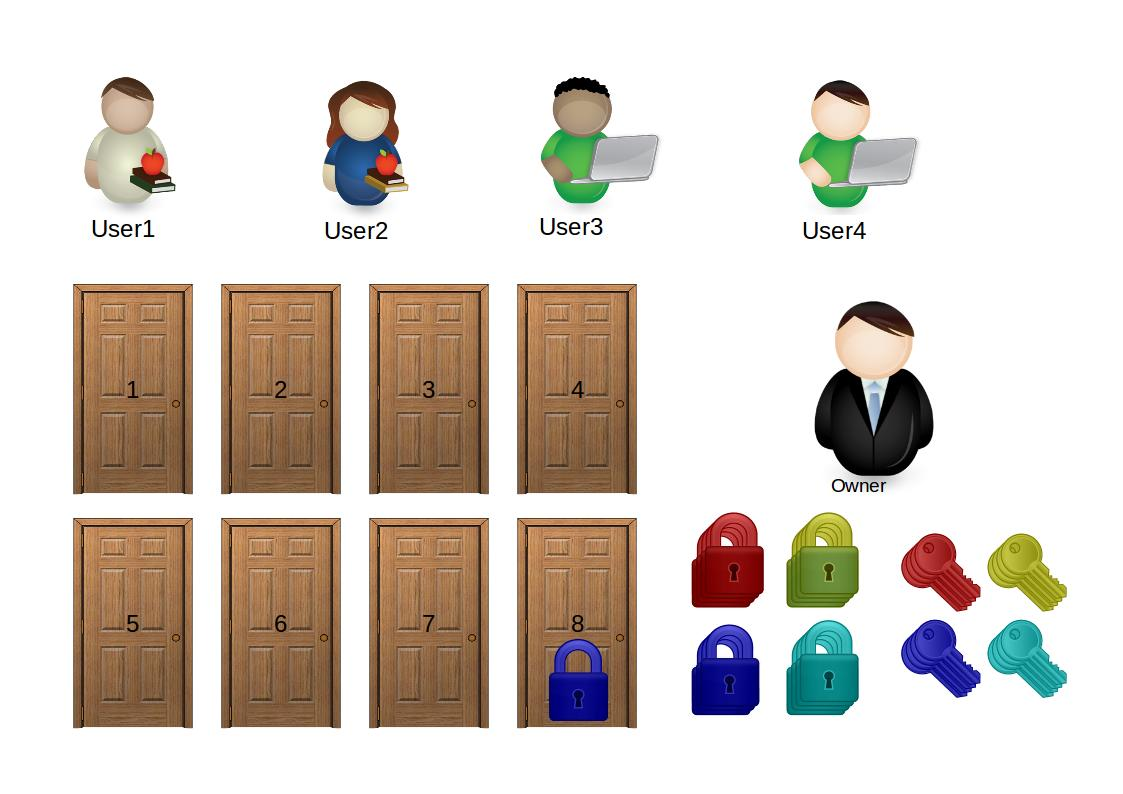
\includegraphics[width=0.7\linewidth]{./media/2}
		\label{fig:2}
	\end{figure}
\end{frame}

\begin{frame}{Specifications}{Concept of locks and keys}
	\textbf{User1 gets access to door 8}
	\begin{figure}
		\centering
		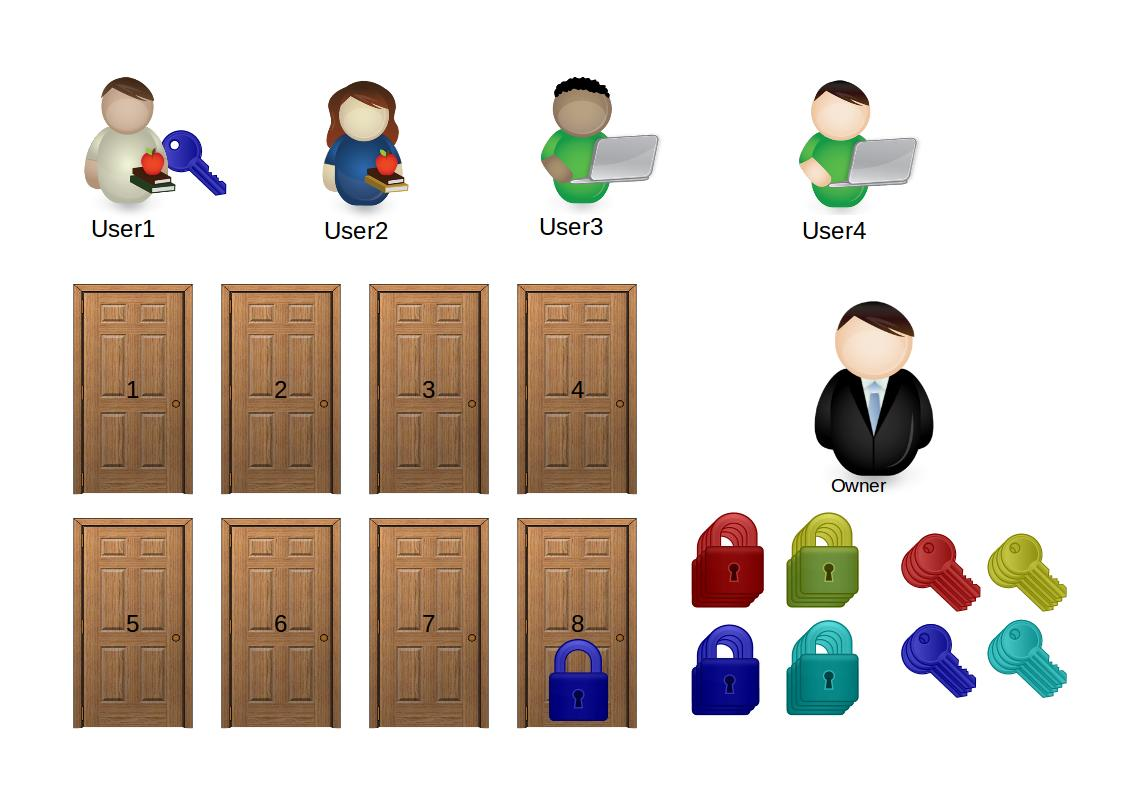
\includegraphics[width=0.7\linewidth]{./media/3}
		\label{fig:3}
	\end{figure}
\end{frame}

\begin{frame}{Specifications}{Concept of locks and keys}
	\textbf{Giving access to other users}
	\begin{figure}
		\centering
		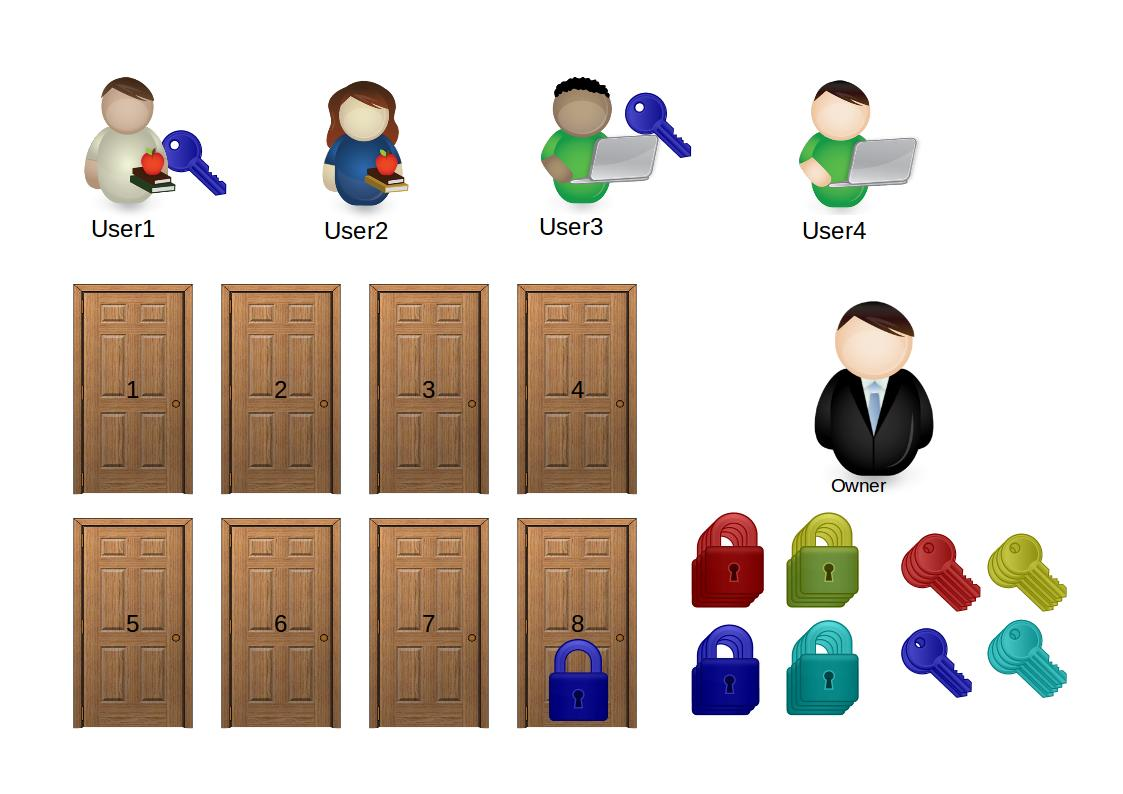
\includegraphics[width=0.7\linewidth]{./media/4}
		\label{fig:4}
	\end{figure}
\end{frame}

\begin{frame}{Specifications}{Concept of locks and keys}
	\textbf{A different type of lock}
	\begin{figure}
		\centering
		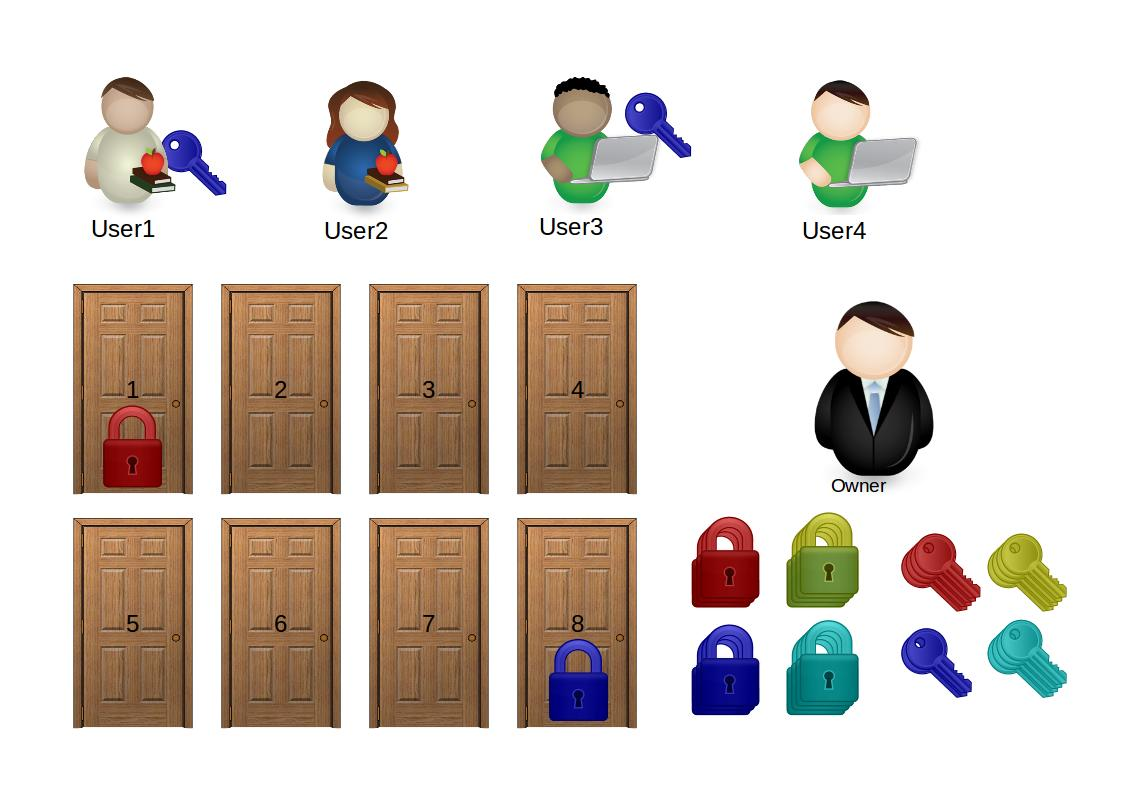
\includegraphics[width=0.7\linewidth]{./media/5}
		\label{fig:5}
	\end{figure}
\end{frame}

\begin{frame}{Specifications}{Concept of locks and keys}
	\textbf{User1 gets access to multiple doors}
	\begin{figure}
		\centering
		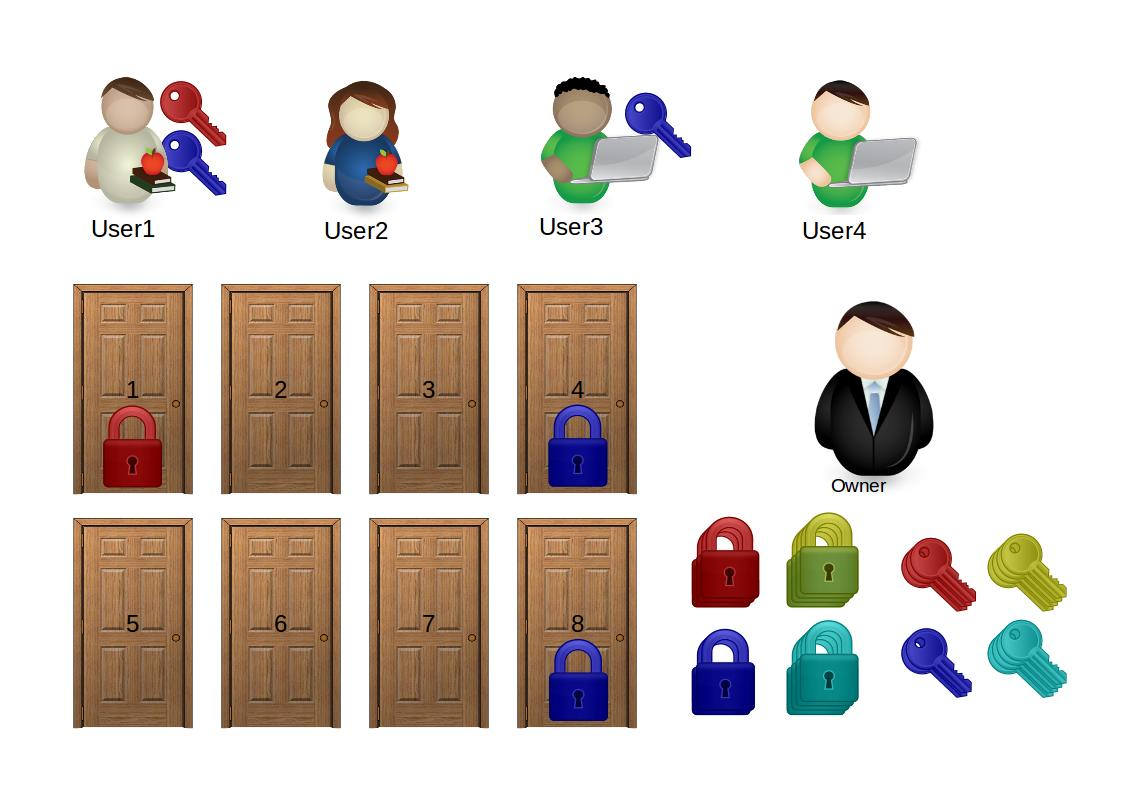
\includegraphics[width=0.7\linewidth]{./media/6}
		\label{fig:6}
	\end{figure}
\end{frame}

\begin{frame}{Specifications}{Concept of locks and keys}
	\textbf{Restricting access by taking away the key}
	\begin{figure}
		\centering
		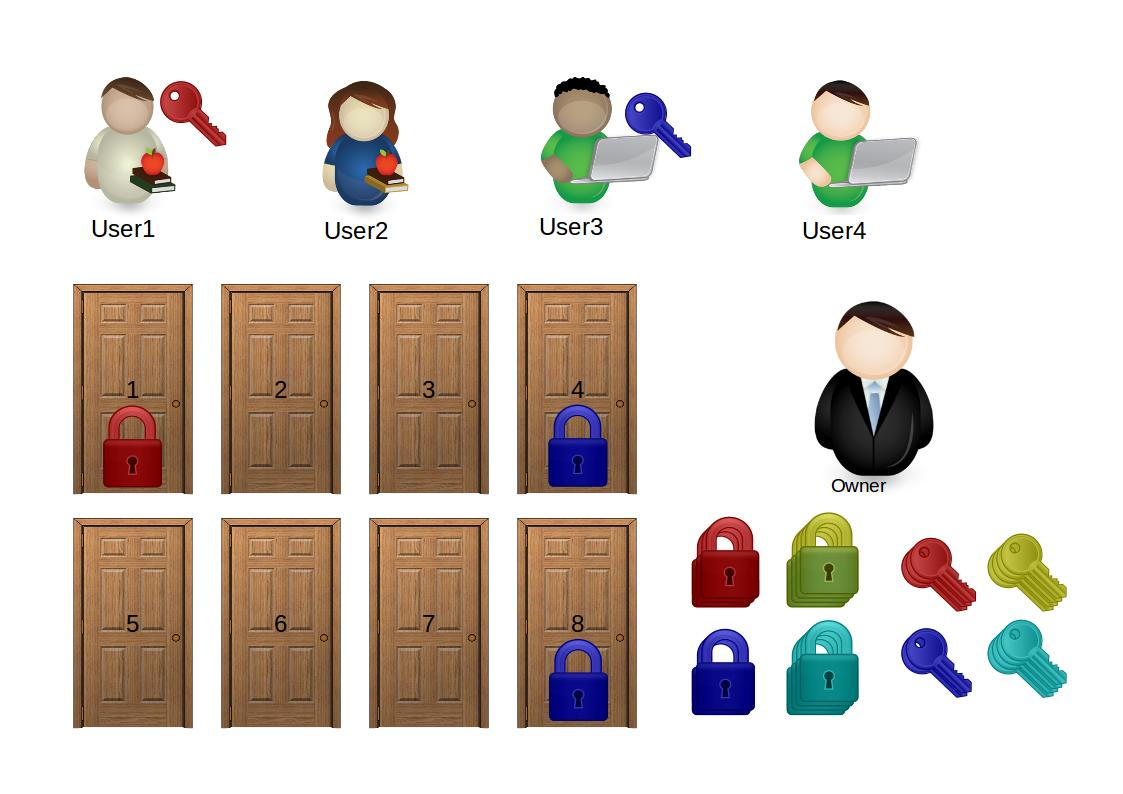
\includegraphics[width=0.7\linewidth]{./media/7}
		\label{fig:7}
	\end{figure}
\end{frame}

\begin{frame}{Specifications}
	\begin{itemize}
		\item Analogy
		\begin{itemize}
			\item Owner: Instructor
			\item Users: Students.
			\item Doors/rooms: Content offered on Bodhitree.
			\item Locks: Tagging of content by an instructor.
			\item Keys: Granting of access to the students for those tags.
		\end{itemize}
		\item Learning elements that can be tagged:
		\begin{itemize}
			\item Videos
			\item Documents
			\item Quizzes
			\item Video markers (In-video Quizzes)
		\end{itemize}
	\end{itemize}
\end{frame}

\begin{frame}{Design}{Defaults}
	\begin{itemize}
		\item When an element (video, document, quiz or video markers) is created in a concept, the default tag is set as \textit{``Free"}
		\item A \textit{``Free''} tag denotes that all the students who are registered for that course can access that element
		\item Fields \textit{premium\_tag} and \textit{premium\_marker} added in the database
	\end{itemize}\vspace{-0.1in}
	\begin{figure}
	\centering
	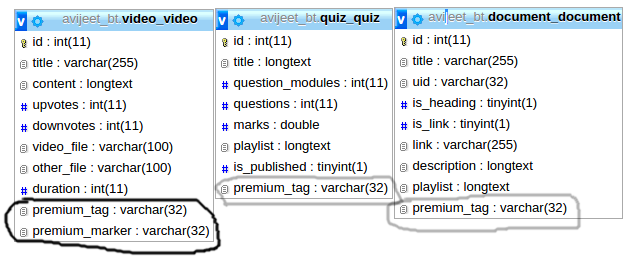
\includegraphics[width=0.7\linewidth]{./media/premium_db1}
	\label{fig:premium_db1}
	\end{figure}
\end{frame}

\begin{frame}{Design}{Tagging interface}
	\begin{figure}
	\centering
	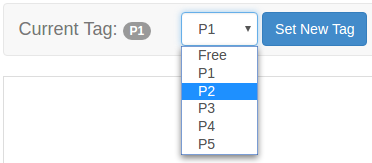
\includegraphics[width=0.5\linewidth]{./media/tag_ui}
	\caption{Tagging interface}
	\label{fig:tag_ui}\vspace{-0.2in}
	\end{figure}
	\begin{itemize}
		\item A badge shows the currently set tag
		\item A drop down box which lists the 5 fixed tags (P1, P2, P3, P4, P5), and the custom tags
		\item Setting a new tag changes the \textit{premium\_tag} field in the database
	\end{itemize}
\end{frame}

\begin{frame}{Design}{Student view}
	\textbf{Student's access to a learning element}
	\begin{figure}
	\centering
	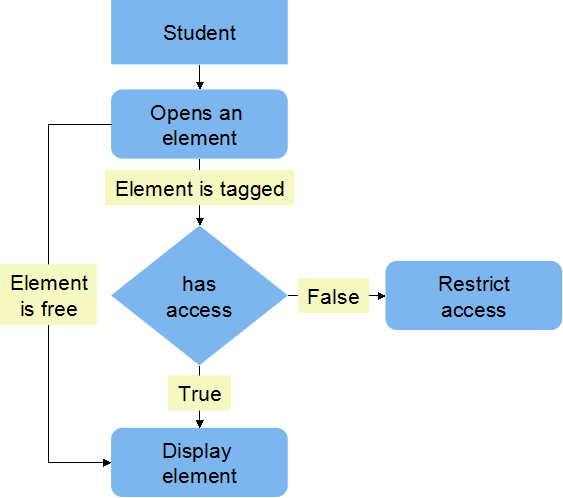
\includegraphics[width=0.6\linewidth]{./media/ACdfd}
	\label{fig:ACdfd}
	\end{figure}
\end{frame}

\begin{frame}{Design}{Student view}
	\begin{itemize}
		\item Server check the user request and sends appropriate data
		\item Data is not sent to unauthorized users
		\item The field \textit{``has\_access''} is set to \textit{false} in the JSON that is fetched, resulting in the following message
	\end{itemize}
	\begin{figure}
	\centering
	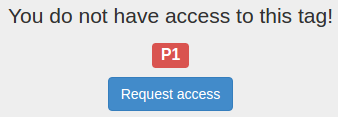
\includegraphics[width=0.5\linewidth]{./media/ac_no}
	\label{fig:ac_no}
	\end{figure}
\end{frame}

\begin{frame}{Design}{Unauthorized access}
	\textbf{Data sent to client who is not having access to an element}	
	\begin{figure}
	\centering
	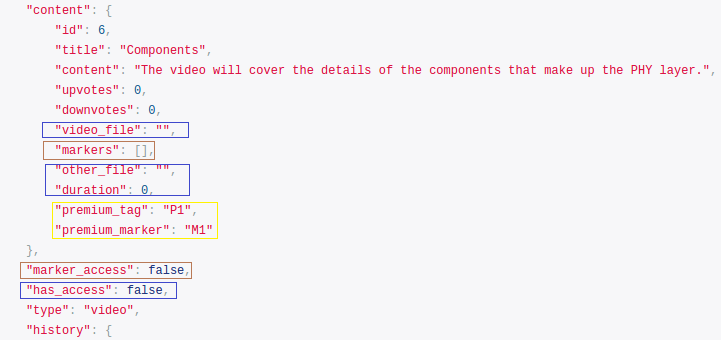
\includegraphics[width=1\linewidth]{media/SUgetdata}
	\label{fig:SUgetdata}
	\end{figure}
\end{frame}

\begin{frame}{Design}{Granting access to users}
	\begin{itemize}
		\item Uploading the CSV file:
		\begin{center}
		\begin{tabular}{|c|c|c|c|}
			\hline stud1 & P1 & P2 & P3 \\ 
			\hline stud2 & P1 &  &  \\ 
			\hline stud3 & P3 &  &  \\ 
			\hline 
		\end{tabular}
		\end{center} 
		\item Checking username against the registered users
		\item Storing the tags in the database: 
		\begin{center}
			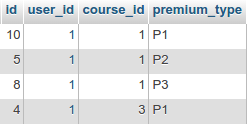
\includegraphics[width=0.5\linewidth]{media/premiumAccesses}
		\end{center}
	\end{itemize}
\end{frame}

\begin{frame}{Design}{CSV file upload}
	Interface to upload the CSV file:
	\begin{figure}
	\centering
	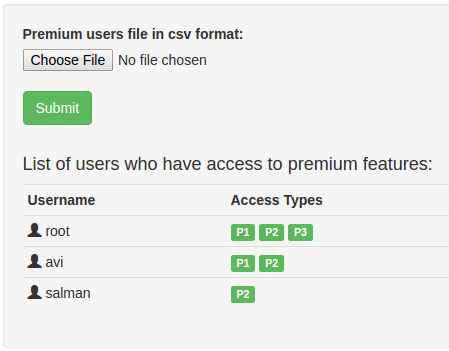
\includegraphics[width=0.6\linewidth]{media/CSVupload}
	\label{fig:CSVupload}
	\end{figure}
\end{frame}

\begin{frame}{Design}{Upload success}
	Information displayed after successfully uploading a CSV file\vspace{-0.1in}
	\begin{figure}
	\centering
	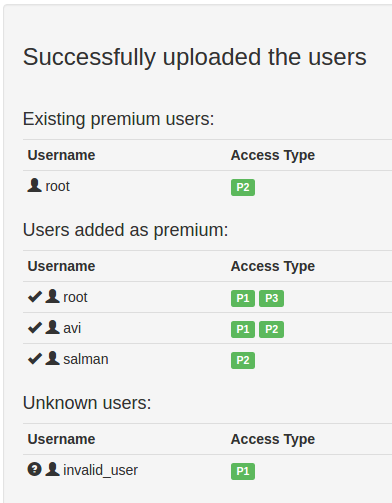
\includegraphics[width=0.4\linewidth]{./media/usertaguploadsuccess}
	\label{fig:usertaguploadsuccess}
	\end{figure}
\end{frame}

\begin{frame}{Design}{Removal of access}
\textbf{Removing of tags access from users}
	\begin{itemize}
		\item Content developer has the authority to remove the tags access
		\item Checklist provided listing the users and associated tags
		\item Corresponding entries removed from the database
	\end{itemize}
\end{frame}

\begin{frame}{Design}{Removal of access UI}
\textbf{Interface to remove tag access}
	\begin{figure}
	\centering
	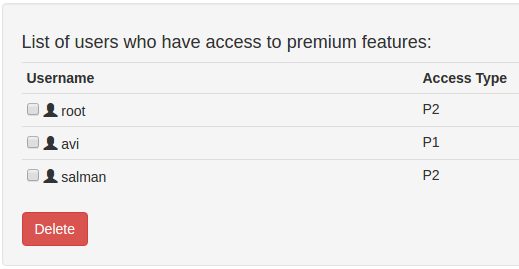
\includegraphics[width=0.6\linewidth]{media/removeusers}
	\label{fig:removeusers}
	\end{figure}
\end{frame}

\begin{frame}{Design}{Custom tags}
\textbf{Creation of custom tags by the instructor}
	\begin{itemize}
		\item If the 5 default tags \textbf{(P1, P2, P3, P4, P5)} are
		not enough, the instructor may create new tags of
		his own
		\item Once created, custom tags ar available in the drop down list of the tagging interface
	\end{itemize}
\end{frame}

\begin{frame}{Design}{Custom tags}
\textbf{Interface for adding custom tags}
	\begin{figure}
	\centering
	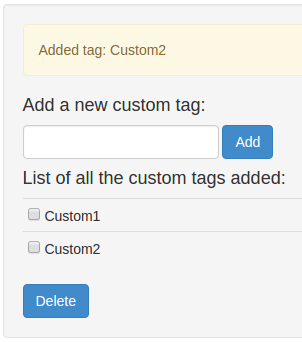
\includegraphics[width=0.3\linewidth]{media/ct_create}
	\label{fig:ct_create}
	\end{figure}
\end{frame}

\begin{frame}{Design}{Custom tags}
\textbf{Custom tags available in the tagging interface after creation}
	\begin{figure}
	\centering
	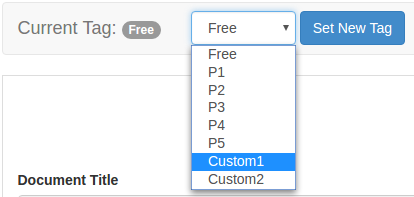
\includegraphics[width=0.5\linewidth]{media/ct_set}
	\label{fig:ct_set}
	\end{figure}
\end{frame}

\begin{frame}{Design}{Group tagging}
\textbf{Tag all the elements (Videos, Documents, etc.) in one click}
	\begin{figure}
	\centering
	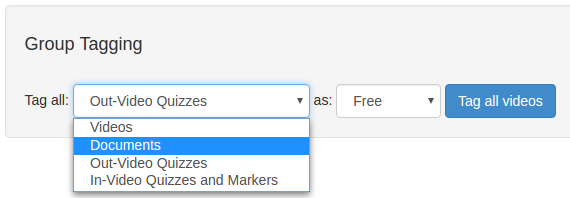
\includegraphics[width=0.6\linewidth]{media/gt1} \\
	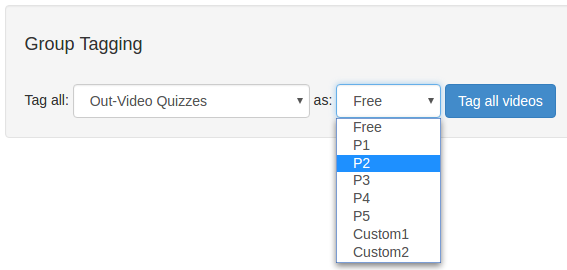
\includegraphics[width=0.6\linewidth]{media/gt2}
	\label{fig:gt}
	\end{figure}
\end{frame}

\section{General}

\subsection{Facebook style notifications}

\begin{frame}{Facebook style notifications}
	\begin{block}{Problem Statement}
	\end{block}
\end{frame}

\subsection{Miscellaneous}

\begin{frame}{Miscellaneous}
	\begin{itemize}
		\item In-Video Quiz ON/OFF
		\item Setting importance to threads
		\item Email instructors on addition of a new thread
	\end{itemize}
\end{frame}

%\subsection*{In-video quiz ON/OFF}
%
%\subsection*{Setting importance to threads}
%
%\subsection*{Email instructors on addition of a new thread}


%\subsection{Another Subsection}
%
%\begin{frame}{Blocks}
%\begin{block}{Block Title}
%You can also highlight sections of your presentation in a block, with it's own title
%\end{block}
%\begin{theorem}
%There are separate environments for theorems, examples, definitions and proofs.
%\end{theorem}
%\begin{example}
%Here is an example of an example block.
%\end{example}
%\end{frame}

% Placing a * after \section means it will not show in the
% outline or table of contents.

\section{Conclusion}

\begin{frame}{Conclusion}
	\begin{itemize}
		\item 
	\end{itemize}
\end{frame}

%\section*{Summary}
%
%\begin{frame}{Summary}
%  \begin{itemize}
%  \item
%    The \alert{first main message} of your talk in one or two lines.
%  \item
%    The \alert{second main message} of your talk in one or two lines.
%  \item
%    Perhaps a \alert{third message}, but not more than that.
%  \end{itemize}
%  
%  \begin{itemize}
%  \item
%    Deficiencies in my work
%    \begin{itemize}
%    \item Emailing instructors on addition of a new thread, good for Bodhi-class, bad for Bodhi-book
%    \item Clearing the notifications is not course specific
%    \end{itemize}
%  \end{itemize}
%  
%\end{frame}



% All of the following is optional and typically not needed. 
\section*{References}

\begin{frame}[allowframebreaks]{References}
    
  \begin{thebibliography}{10}

  \bibitem{flipped}
  	The University of Texas at Austin: \small
  	Faculty Innovation Center
    \newblock  \small \url{https://facultyinnovate.utexas.edu/teaching/flipping-a-class}
 
%  \bibitem{Someone2000}
%    S.~Someone.
%    \newblock On this and that.
%    \newblock {\em Journal of This and That}, 2(1):50--100,
%    2000.
  \end{thebibliography}
\end{frame}

\end{document}